\section{Durchführung}
\label{sec:Durchfuehrung}
\begin{figure}
	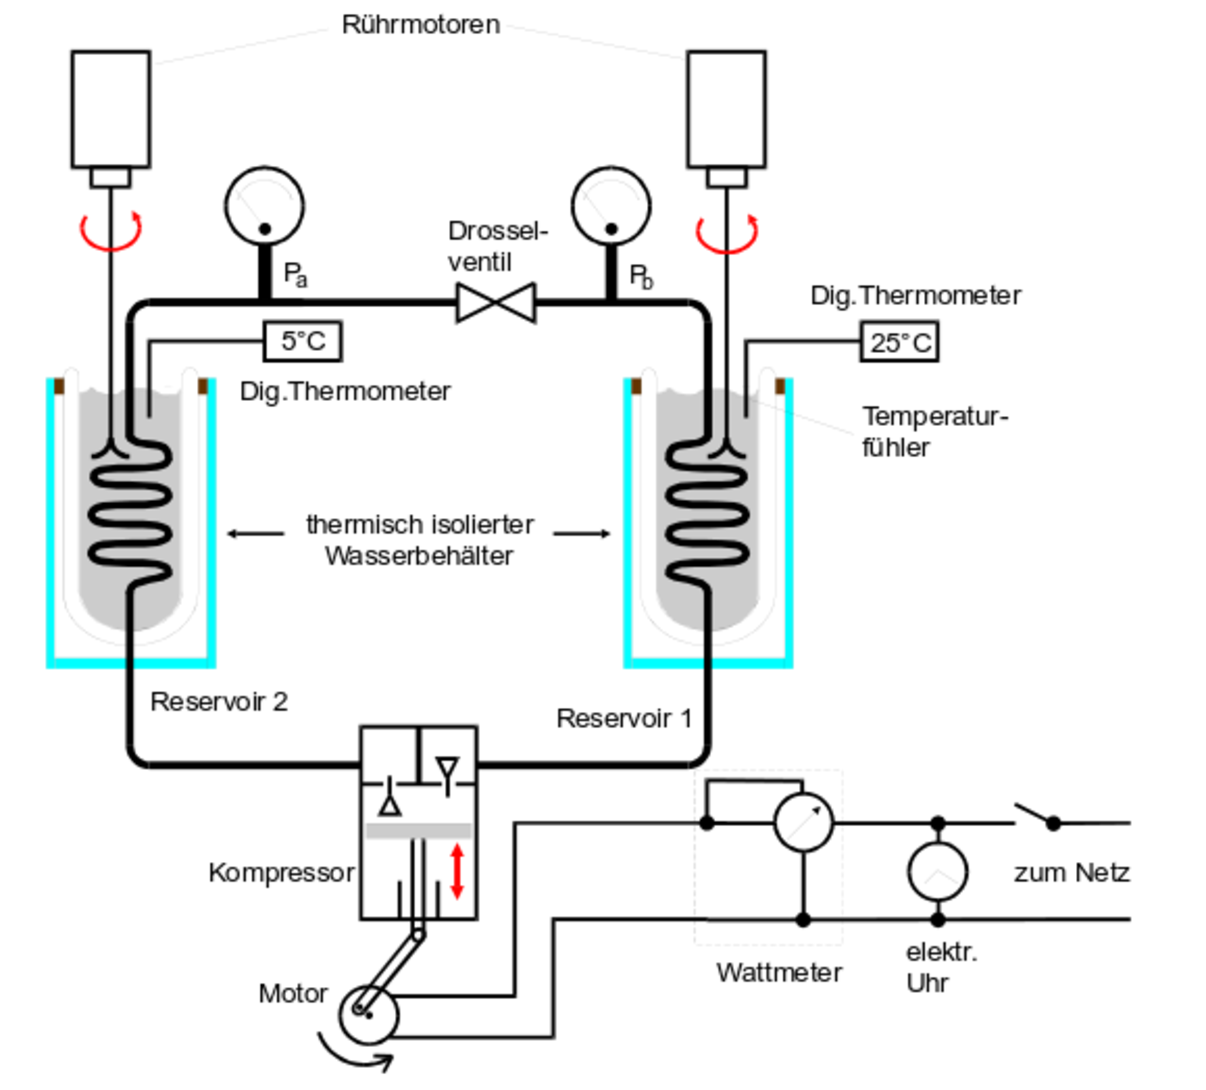
\includegraphics[width=\textwidth]{Bilder/Abbildung.pdf}
	\caption{Schematischer Aufbau der Wärmepumpe \cite{V206}}
	\label{fig:pumpe}
\end{figure}
Die verwendete Wärmepumpe ist in Abbildung \ref{fig:pumpe} dargestellt.
Durch das geschlossene System fließt eine Medium mit hoher Kondensationswärme, der Fluorchlorkohlenwasserstoff \textit{R12}.
Das Medium verdampft in der Kupferspirale im kälteren Reservoir bei geringem Druck $p_\text{k}$ und wird im Kompressor adiabatisch komprimiert. 
Das Gas wird unter höherem Druck $p_\text{w}$ zum warmen Reservoir geführt und kondensiert in dessen Kupferspirale unter Abgabe der aufgenommenen Energie $Q_2+A$.
Das Drosselventil sorgt für einen Druckunterschied im Kreislauf, sodass die Flüssigkeit erneut unter dem geringerem Druck $p_\text{w}$ in der Kupferspirale des kälteren Reservoirs verdampft. 
Die Reservoire und die Verbindungsleitungen sind thermisch isoliert, sodass das Wärmepumpensystem abgesehen durch die Kupferspiralen keine Wärme nach außen abgibt.
Während der Messung wird der Inhalt der Reservoire mittels Rührer durchmischt.

Der Kompressor bezieht Energie aus dem Netz, die Leistung $P_\text{el.}$ des Kompressors wird von einem Wattmeter angezeigt. 
Die Temperatur $T_\text{k}$ und $T_\text{w}$ der Reservoire und die Drücke $p_\text{k}$ und $p_\text{w}$ in den Kupferspiralen ist per Messinstrumente ablesbar.

Es wird in den Reservoiren jeweils 3 Liter Leitungswasser mit gleicher Temperatur gefüllt und die Parameter $p_\text{k}$, $p_\text{w}$, $T_\text{k}$, $T_\text{w}$ sowie die Leistungsaufnahme des Kompressors $P_\text{el}$ pro Minute aufgenommen, bis das wärmere Reservoir eine Temperatur von $50\si{\degreeCelsius}$ erreicht.